\documentclass[10pt,a4paper]{article}
\usepackage[utf8]{inputenc}
\usepackage[german]{babel}
\usepackage[T1]{fontenc}
\usepackage{graphicx}

\usepackage[paper=a4paper,width=14cm,left=35mm,height=22cm]{geometry}
\usepackage{setspace}
\usepackage{acronym}
\usepackage{charter}
\linespread{1.15}
\setlength{\parskip}{0.25em}
\setlength{\parindent}{0em}

\bibliographystyle{apalike} 

\begin{document}
\author{Markus Tacker}
\title{Konzepte und Standards zur domänenübergreifenden Integration von komplexen Webanwendungen}
\maketitle
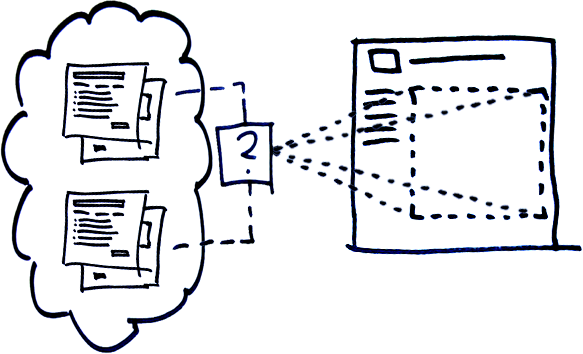
\includegraphics{skizze.png}
Ein Teil der neueren Entwicklung des Internets zum \emph{Web 2.0} basiert auf der Idee, dass Informationen und Funktionen von Software mit Hilfe von \emph{Webservices} verwendet werden können. \cite{hn-web20}

Die Kommunikation mit Webservices ist zwar auf Protokollebene standardisiert (siehe \ref{l:wsprot}), muss jedoch vom Konsumenten immer individuell entsprechend dem Domänenmodell des Anbieters implementiert werden, wodurch eine feste Bindung an den Anbieter entsteht.

Für sogenannte \emph{Blackbox-Webservices}~(siehe~\ref{l:blackbox}) ist das kein Problem --- diese zustandslose Dienste verarbeiten lediglich einfache Daten, d.h. dass der Dienst durch Übergabe eines Datums aufgerufen wird, dieser entsprechend des Aufrufs reagiert und ein Ergebnis zurück liefert.

Anbieter \emph{webbasierter Anwendungen}~(siehe~\ref{l:webanw}) stehen jedoch vor dem Problem, dass auf Seiten des Anbieters komplexe Arbeitsabläufe abgebildet werden und diese auch persistent innerhalb des Dienstes verbleiben, d.h. sie sind zustandsbehaftet. Auch hier bietet sich die Möglichkeit der Anbindung mittels Schnittstellen, jedoch mit deutlich gesteigertem Aufwand, da zwischen beiden Parteien das Verständnis über die verarbeiteten Entitäten vermittelt werden muss. 

Nach \cite[Seite 653]{ei-sawsdl} sind etablierte Standards für Webservices der ersten Generation wie \acs{SOAP} und \acs{UDDI} primär unter dem Aspekt entwickelt worden, einen einfachen Weg zur Verteilung und Wiederverwertung von Webservices zu etablieren --- ihnen fehlt also eine Standardisierung für das Auffinden, Zusammenstellen und Auswählen von Diensten um eine \emph{lose Kopplung}~(Siehe~\ref{l:loosec}) zu ermöglichen. Für ein lebendiges Web-Öko-System ist die lose Kopplung jedoch von entscheidender Bedeutung --- im Idealfall lassen sich Dienste so anbinden, dass sie jederzeit und ohne Aufwand ausgetauscht werden könen und sogar die parallele Verwendung mehrere Dienste der gleichen Art ermöglicht wird.

\textbf{In dieser Seminararbeit möchte ich versuchen die Frage zu beantworten, welche Konzepte für die dynamische Bindung von komplexen Webanwendungen existieren.}

\pagebreak

\tableofcontents

\pagebreak

\section{Einleitung}

\subsection{Problemstellung}
\begin{itemize}
\item "Whitebox"-Anbindung
\item Bisher: 1:1-Verbindung (Beispiel Mite)
\item Problem Ontologie. Projekt = Was?
\end{itemize}
\subsection{Beispiele}
\begin{itemize}
\item Mite
\item E-Mail-Backup
\end{itemize}
\subsection{Definition}
\subsection{Webservice-Protokolle}
\label{l:wsprot}
\subsection{Blackbox-Dienste}
\label{l:blackbox}
Für die Nutzung eines Dienstes reicht die Kenntnis der Schnittstellen aus. Ein tieferes Verständnis
der internen Vorgänge wird nicht benötigt, bzw. soll bewusst verborgen werden. \cite{hhxmlwssoa}

Beispiele hierfür ist z.B. ein Webservice, der Wetterdaten für eine PLZ liefert. Hier gibt der Konsument die PLZ eines Ortes in Deutschland ein und erhält in der Antwort eine Temperatur. Die genauen technischen Abläufe, wie der Webservice aus der PLZ eine Temperatur ermittelt bleiben für den Konsumenten verborgen und sind für diesen auch irrelevant.

Diese Arten von Diensten sind zustandslos, d.h. sie behandlen jede Anfrage unabhängig von einer vorherigen.
\subsection{Webbasierte Anwendungen, Whitebox-Dienste}
\label{l:webanw}
Nicht zustandslos.

Beispiele hierfür sind z.B. Werkzeuge zur projektspezifischen Zeiterfassung. 
\paragraph{Loose Kopplung}
\label{l:loosec}

\section{Semantische Webservices}

\subsection{Problemstellung}

\subsection{...}

\subsection{Beispiele}

\paragraph{Webintents}

\paragraph{OpenSearch}

\section{Fazit und Ausblick}

\pagebreak

\subsection*{Abkürzungsverzeichnis}
\begin{acronym}
\acro{SOAP}{Simple Object Access Protocol}
\acro{UDDI}{Universal Description, Discovery and Integration}
\end{acronym}

\bibliography{bibliothek}
\end{document}